\documentclass[a5paper,pagesize]{scrbook}

\usepackage[T1]{fontenc}
\usepackage[utf8]{inputenc}

\usepackage{amssymb}
\usepackage{authblk}
\usepackage[ngerman]{babel}
\usepackage[natbib,notes,backend=bibtex]{biblatex-chicago}
   \bibliography{references}
\usepackage{booktabs}
\usepackage{CormorantGaramond}
\usepackage[german=guillemets]{csquotes}
\usepackage{enumitem}
   \setlist{noitemsep}
\usepackage{float}
\usepackage{graphicx}
   \graphicspath{{figures/}}
\usepackage[hidelinks]{hyperref}
   \urlstyle{same}
\usepackage{longtable}
\usepackage{microtype}
\usepackage{siunitx}
\usepackage{tabto}
\usepackage{tikz}
\usepackage{ulem}
\usepackage{url}

\addtokomafont{disposition}{\rmfamily}

\setlength{\fboxsep}{0pt}
\setlength{\fboxrule}{1pt}

\deffootnote{1.5em}{1em}{\makebox[1.5em][l]{\thefootnotemark}}
   \setlength{\skip\footins}{1.5em}
   \setlength{\footnotesep}{1em}

\title{Gothic}
\subtitle{}

\author{Alexander Max Bauer}

\date{}


%%%%%%%%%%%
% TITELEI %
%%%%%%%%%%%
\begin{document}
\maketitle


%%%%%%%%%%%%%%%%%%%%%%
% INHALTSVERZEICHNIS %
%%%%%%%%%%%%%%%%%%%%%%
\frontmatter
\tableofcontents


%%%%%%%%%%%
% VORWORT %
%%%%%%%%%%%
\chapter{Vorwort}


%%%%%%%%%%%
% ORPHEUS %
%%%%%%%%%%%
\mainmatter
\chapter{Orpheus -- Ein Gefängnis in Planung}\label{ch:orpheus}
Gothic hieß nicht immer Gothic.
Der erste Name, den das Projekt trug, war \textit{Orpheus}. % Mike Hoge fragen, woher der Name stammt.
Aus dieser frühen Phase -- wir sprechen grob von den Jahren 1995 und 1996 -- ist eine Handvoll Dokumente erhalten, in denen Mike Hoge erste Ideen festgehalten hat.\footnote{Diese Dokumente wurden den Betreibern des \textit{Gothic Archives} von Mike Hoge zur Verfügung gestellt, die sie anschließend digitalisiert und online zugänglich gemacht haben (vgl. \autocite{archive_orpheus}).}
Sie lassen sich anhand einiger in ihnen enthaltener Titel grob gliedern:

\begin{itemize}
   \item \enquote{\uline{Aufträge}}\autocite[S.~16--17]{orpheus_b_scribbles}
   \item \enquote{\uline{\textsc{Der rote Faden...}}}\autocite{orpheus_der_rote}
   \item \enquote{\uline{Der Werdegang eines SC's}}\autocite{orpheus_der_werdegang}
   \item \enquote{\uline{\textsc{Orpheus -- Bewegungen}}}\autocite{orpheus_bewegungen}
   \item \enquote{\textsc{Orpheus -- History}}\autocite[S.~2--3]{orpheus_b_scribbles}
   \item \enquote{\uline{\textsc{Orpheus} -- Interface}}\autocite{orpheus_interface}
   \item \enquote{\textsc{Orpheus -- Kreaturen}}\autocite[S.~4]{orpheus_b_scribbles}
   \item \enquote{\textsc{Orpheus -- Locations}}\autocite[S.~5]{orpheus_b_scribbles}
   \item \enquote{\textsc{Orpheus} -- Spielwelt/Gildensystem}\autocite{orpheus_gildensystem}
   \item \enquote{\textsc{Orpheus} -- Spielwelt/Gildensystem V2}\autocite{orpheus_gildensystem_v2}
   \item \enquote{\textsc{Orpheus} -- \uline{Übersicht}}\autocite[S.~11--14]{orpheus_b_scribbles}
   \item \enquote{Zusammenfassung zum Orpheus-Konzept. \uline{Graphiken}}\autocite{orpheus_zusammenfassung}
\end{itemize}

\noindent Daneben gibt es noch ein Dokument zur Kampfsteuerung,\autocite{orpheus_kampfsteuerung} das -- abgesehen von den Überschriften seiner einzelnen Abschnitte -- keinen eigenen Titel trägt, sowie einige lose Notizen, die sich neben den oben genannten Titeln \enquote{\textsc{History}}, \enquote{\textsc{Kreaturen}}, \enquote{\textsc{Locations}}, \enquote{\uline{Übersicht}} und \enquote{\uline{Aufträge}} in einem Konvolut finden, dem ein Deckblatt mit der Aufschrift \enquote{\textsc{Orpheus. B -- Scribbles}} vorangestellt ist.\autocite{orpheus_b_scribbles}

Bei der \enquote{Zusammenfassung zum Orpheus-Konzept} handelt es sich vermutlich um ein ursprünglich umfangreicheres Dokument, von dem nur noch der Abschnitt zu \enquote{\uline{Graphiken}} erhalten geblieben ist.\autocite[Vgl.][]{archive_orpheus}
Es steht vermutlich nicht nur alphabetisch am Ende:
Die Zusammenfassung -- oder was von ihr übrig ist -- stellt das einzige nicht handschriftlich verfasste Schriftstück in der Sammlung dar und ist auf den 12. Dezember 1996 datiert.
Die anderen Dokumente sollten dementsprechend etwas älter sein; der in ihnen enthaltene Entwurf einer Karte wird beispielsweise auf das Vorjahr, also 1995, geschätzt.\autocite{flosha_evolution}

Im Folgenden werfen wir einen genaueren Blick auf diese Dokumente, die ich dafür der Übersichtlichkeit halber grob in thematische Gruppen gliedere, wobei es natürlich Überschneidungen und unscharfe Grenzen gibt.
Den Anfang machen Überlegungen zur Darstellung (\autoref{sec:orpheus_darstellung}), gefolgt von Ideen zur Spielmechanik und Steuerung (\autoref{sec:orpheus_mechanik}) sowie zur Geschichte des Spiels (\autoref{sec:orpheus_geschichte})...


%%%%%%%%%%%%%%%%%%%%%%%%%
% ORPHEUS – DARSTELLUNG %
%%%%%%%%%%%%%%%%%%%%%%%%%
\section{Darstellung}\label{sec:orpheus_darstellung}
Drei der oben genannten Schriftstücke befassen sich mit Überlegungen zur Darstellung des Spiels:
\enquote{\uline{\textsc{Orpheus -- Bewegungen}}}, \enquote{\uline{\textsc{Orpheus} -- Interface}} sowie das Überbleibsel aus der \enquote{Zusammenfassung}.

Die \enquote{\uline{\textsc{Bewegungen}}} umfassen eine mit Bleistift beschriebene Blankoseite sowie drei mit Fineliner beschriebene Karoseiten.
Das \enquote{\uline{Interface}} wiederum besteht aus sieben mit Kugelschreiber und Fineliner beschrifteten Blankoseiten.
Aus der \enquote{Zusammenfassung zum Orpheus-Konzept} schließlich ist nur ein dreiseitiger, am Computer verfasster Teil zu \enquote{\uline{Graphiken}} erhalten, der seinerseits unterteilt ist in die Abschnitte \enquote{\uline{Spielansicht}}, \enquote{\uline{Spielfigurenanimation}}, \enquote{\uline{Getrennt animierte GAMS}}, \enquote{\uline{Diverse Mashes}}, \enquote{\uline{Texturen}} sowie \enquote{\uline{Evtl. User\-Controlled-Online-Animation}}.

Auf diesen Seiten finden wir unter anderem Informationen hinsichtlich geplanter Kameraperspektiven (\autoref{sec:orpheus_darstellung_kamera}), technischer Überlegungen zu Animationen (\autoref{sec:orpheus_darstellung_animation}), des von ihnen abgebildeten Bewegungsumfangs (\autoref{sec:orpheus_darstellung_bewegungsumfang}), der Realisation einer hohen Figurenvielfalt (\autoref{sec:orpheus_darstellung_figurenvielfalt}) sowie der Umsetzung des Inventars (\autoref{sec:orpheus_darstellung_inventar}).


%%%%%%%%%%%%%%%%%%%%%%%%%%%%%%%%%%
% ORPHEUS – DARSTELLUNG – KAMERA %
%%%%%%%%%%%%%%%%%%%%%%%%%%%%%%%%%%
\subsection{Kamera}\label{sec:orpheus_darstellung_kamera}
In der \enquote{Zusammenfassung} ist unter der Überschrift \enquote{\uline{Spielansicht}}\autocite[Vgl.][S.~1]{orpheus_zusammenfassung} festgehalten, dass zu dieser Zeit insgesamt drei verschiedene Kameraperspektiven vorgesehen waren.
Während des Spielens hätten Spieler*innen frei zwischen Ego- und Verfolgerperspektive wählen können sollen, wobei für letztere vorgesehen war, dass sich die Kamera etwa fünf Meter hinter der Spielfigur befindet und mit Wänden kollidiert:
\enquote{Steht die Figur mit dem Rücken zur Wand, sieht ihr die Kamera über die Schulter. Geht die Figur jetzt los[,] so folgt ihr die Kamera erst wieder, wenn die Figur 5m entfernt ist.}
Eine dritte Variante war für den \enquote{Kampfmodus} (siehe auch \autoref{sec:orpheus_mechanik}) vorgesehen:

\begin{quote}
Ist die Figur im Kampfmodus $[\dots]$ und ist sie in Reichweite eines Monsters $[\dots]$, so dreht sich die Kamera 90$^\circ$ gegen den Uhrzeigersinn. Die Kontrahenten werden jetzt von der Seite gezeigt. Ist der Kampf vorbei, so sieht man die Figur wieder von hinten.
\end{quote}


%%%%%%%%%%%%%%%%%%%%%%%%%%%%%%%%%%%%%
% ORPHEUS – DARSTELLUNG – ANIMATION %
%%%%%%%%%%%%%%%%%%%%%%%%%%%%%%%%%%%%%
\subsection{Animation}\label{sec:orpheus_darstellung_animation}
Jede (menschliche) Figur, erfahren wir in der \enquote{Zusammenfassung} unter \enquote{\uline{Spiel\-figurenanimation}},\autocite[Vgl.][S.~1]{orpheus_zusammenfassung} sollte aus 15 sogenannten \enquote{\textbf{Limbs}} bestehen, \enquote{einzelnen starren Körperbestandteilen}, die jeweils \enquote{als ein festes Drahtgittermodell [abgespeichert]} und über \enquote{\textit{Anschlußpunkte}} miteinander verbunden werden sollten.
Vorgesehen waren dafür \enquote{Kopf, Oberkörper, Unterleib, 2 Oberarme, 2 Unterarme, 2 Hände, 2 Oberschenkel, 2 Unterschenkel, 2 Füße}.
Visualisiert ist das in \autoref{fig:orpheus_spielfigurenanimation} oben, wobei die schraffierten Flächen die Anschlusspunkte darstellen.
Jede Animationsphase einer solchen Figur sollte \enquote{aus einem Gelenk-Animations-Modell (\textbf{GAM})} bestehen, das sich aus \enquote{19 Raumkoordinaten} sowie \enquote{15 Limbvektoren} zusammensetzt, wobei gelten sollte: \enquote{Jede Koordinate legt eine Gelenkverbindung zwischen zwei Limbs fest.}
Hält die Figur eine Waffe in der Hand, sollte eine zusätzliche Raumkoordinate an deren äußerem Ende (beispielsweise der \enquote{Schwertspitze}) sowie ein zusätzlicher Waffenvektor hinzukommen.
Dargestellt ist das in \autoref{fig:orpheus_spielfigurenanimation} unten links.
Die insgesamt 15 Limbs sind hier über 14 Gelenkverbindungen miteinander verknüpft.
Um auf die 19 -- beziehungsweise mit gezogener Waffe 20 -- Raumkoordinaten zu kommen, braucht es also mehr als nur die Gelenkverbindungen zwischen den Limbs.
Tatsächlich kommen, wie aus der Abbildung deutlich wird,\autocite[Vgl.][S.~3]{orpheus_zusammenfassung} bei Händen, Füßen und Kopf jeweils zusätzliche Punkte hinzu, nämlich \enquote{Zehen}, \enquote{Handfläche} sowie \enquote{Höchster Kopfpunkt}.
Im Spiel sollte die Figur dann \enquote{aus GAM und Limbs \textbf{zusammengesetzt}} werden.
Als \enquote{\uline{Vorteile}} führt Mike Hoge auf:

\begin{quote}
   Jedes Limb muß nur einmal als Mesh abgespeichert werden und kann innerhalb einer Animation immer wieder benutzt werden.
   Somit wird eine angestrebte Vielzahl von Bewegungsabläufen und Animationsschritten bei vergleichsweise geringem Speicheraufwand ermöglicht.
   Es ist möglich, einer Spielfigur den Kopf abzuhacken, so daß er lustig durch die Gegend fliegt.
\end{quote}

Unter \enquote{\uline{Getrennt animierte GAMS}}\autocite[Vgl.][S.~2]{orpheus_zusammenfassung} ist notiert, dass ein Gelenk-Animations-Modell aus vier einzelnen Segmenten bestehen sollte: (1) \enquote{Beine und Unterleib}, (2) \enquote{Oberkörper und Kopf} sowie (3) \enquote{rechter Arm (Aktionsarm)} und \enquote{linker Arm (passiver Arm)}.
Auch dieses Vorgehen bringt einige \enquote{\uline{Vorteile}} mit sich:

\begin{quote}
   Die Figur kann gleichzeitig gehen und schlagen.
   Sie kann mit dem rechten Arm schlagen, den Kopf in die Richtung drehen \sout{und mit links einen Schlag automatisch verteidigen.}
   Wenn die Figur ein Schwert trägt und geht, so bewegt sich der Arm anders als wenn sie mit leeren Händen läuft; die Beinanimation bleibt aber gleich.
   Der linke Arm kann außerdem noch einen Schild tragen und entsprechend animiert sein.
   Der modulare Zusammenbau dieser Animationssequenzen verhindert einen GAM-Overkill, da angestrebt wird, Waffen in der Hand auch im Outsideview darzustellen.\footnote{Die Durchstreichung ist nachträglich handschriftlich erfolgt.}
\end{quote}

Über den letzten animationsbezogenen Punkt, der am Ende der \enquote{Zusammenfassung} steht, die \enquote{\uline{User-Controlled-Online-Animation}},\autocite[Vgl.][S.~3]{orpheus_zusammenfassung} gibt das Dokument keinen Aufschluss mehr. % Mike Hoge fragen.
Es endet mit dem in Klammern gesetzten Kommentar: \enquote{hierzu später mehr, ich muß jetzt Tombraider [sic] spielen}.
Der erste Teil der Tomb-Raider-Serie war keine zwei Monate vorher erschienen, am 25. Oktober 1996.

\vfill
\begin{figure}[p]
   \centering
   \fbox{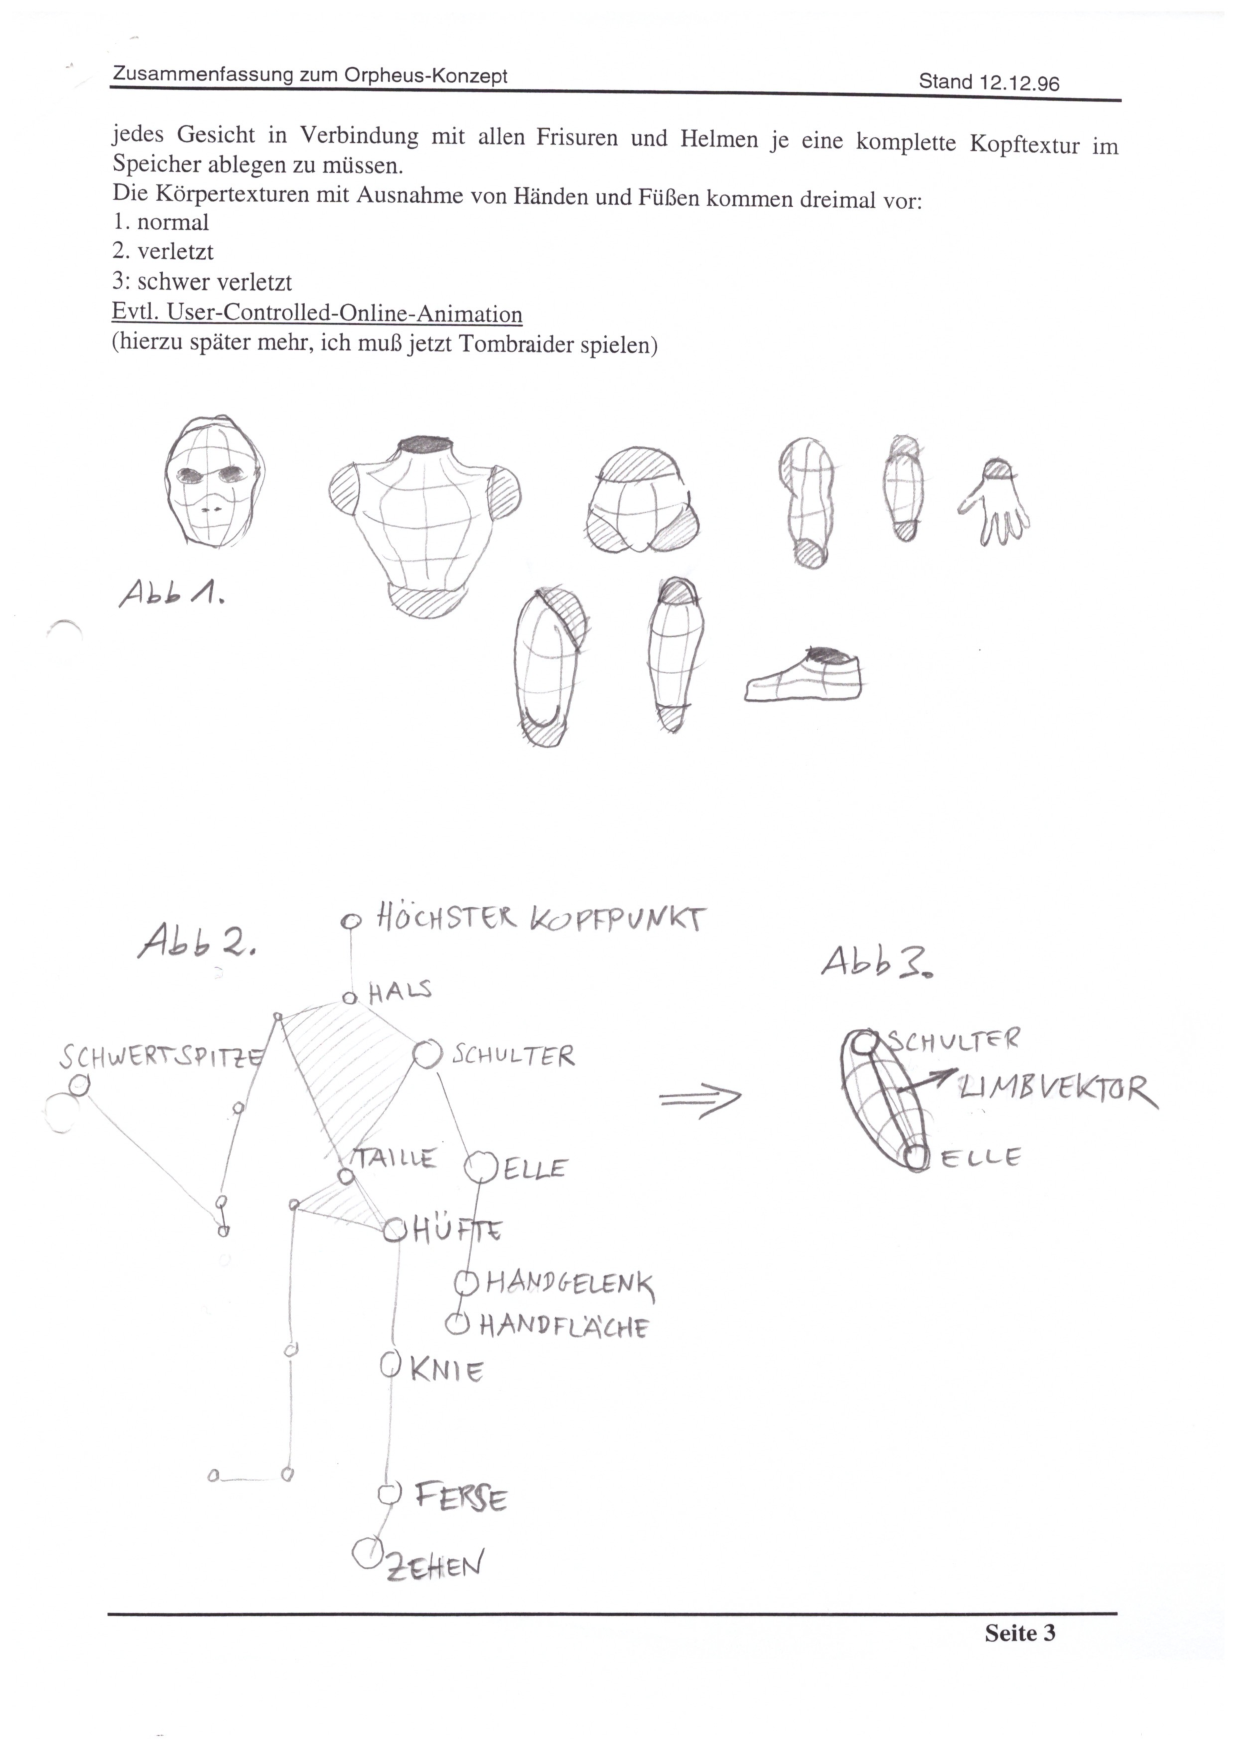
\includegraphics[scale=0.5]{orpheus_spielfigurenanimation.pdf}}
   \caption{Ausschnitt aus \enquote{Zusammenfassung zum Orpheus-Konzept}}
   \label{fig:orpheus_spielfigurenanimation}
\end{figure}


%%%%%%%%%%%%%%%%%%%%%%%%%%%%%%%%%%%%%%%%%%%
% ORPHEUS – DARSTELLUNG – BEWEGUNGSUMFANG %
%%%%%%%%%%%%%%%%%%%%%%%%%%%%%%%%%%%%%%%%%%%
\subsection{Bewegungsumfang}\label{sec:orpheus_darstellung_bewegungsumfang}
Auf der ersten Seite von \enquote{Orpheus -- Bewegungen} finden wir insgesamt 17 Spiegelstriche mit geplanten Animationen und der Information, in wieviele Phasen diese jeweils unterteilt sein sollten.\footnote{Vgl. \autocite[S.~1]{orpheus_bewegungen}. Einen Vergleich zu den im fertigen Spiel enthaltenen Animationen ermöglicht die \textit{Marvin-Datenbank}, deren Zweck es ist, den Testmodus von Gothic (den sogenannten \textit{Marvin Mode}) zu dokumentieren (vgl. \autocite{sillus_marvin}).}
An oberster Stelle steht beispielsweise \enquote{Einhand Angriff × [2] (7 Pha)}.
Geplant waren also vermutlich zwei Varianten eines Angriffs mit einer einhändig geführten Waffe (vielleicht ein Streich von links nach rechts und ein zweiter von rechts nach links), die jeweils sieben Animationsphasen umfassen sollten.
Daneben gibt es hier unter anderem \enquote{Zweihand Angriff}, \enquote{Armbrust}, \enquote{Bogen}, \enquote{getroffen werden} und \enquote{umfallen}, \enquote{mag. offensiv} und \enquote{mag. defensiv} sowie \enquote{stehen}, \enquote{gehen}, \enquote{geduckt gehen}, \enquote{rennen}, \enquote{klettern}, \enquote{Schwimmen} und \enquote{Springen (gehend wie stehend)}, aber auch \enquote{rennend}.

Auf den folgenden -- wahrscheinlich später entstandenen -- drei Seiten wird diese Liste dann unter anderem um \enquote{Dialoggesten} ergänzt und wesentlich ausdifferenziert, insbesondere für Kampfanimationen und Bewegungen mit gezogener Waffe.\autocite[Vgl.][S.~2--4]{orpheus_bewegungen}
Hier tauchen dann neben dem Ziehen der Waffe (\enquote{Draw}, \enquote{Bogen ziehen}, \enquote{Armbrust anlegen}) sowie der \enquote{At[tacke]} und der \enquote{Pa[rade]} unter anderem auch \enquote{Kür}, \enquote{Unterschläge} sowie \enquote{Ruhehaltung} beziehungsweise \enquote{Standpose} auf und das Bewegungsrepertoire wird um das Umdrehen (\enquote{Turn}) sowie um Seitwärtsbewegungen (\enquote{Strafe}) erweitert.
Ein Stichwort fällt besonders ins Auge:
An drei Stellen notiert Mike Hoge \enquote{Threaten \& Kill, Xena-Move}.
Dabei bezieht er sich vermutlich auf die kampferprobte Protagonistin der zwischen 1995 und 2001 gedrehten Fernsehserie \textit{Xena -- Die Kriegerprinzessin}, wobei nicht klar ist, welcher ihrer \enquote{Moves} hier gemeint ist. % Mike Hoge fragen.

Eine ähnliche Auflistung geplanter Animationen finden wir in der \enquote{Zusammenfassung} am Ende des Abschnitts zur \enquote{\uline{Spielfigurenanimation}} (siehe \autoref{sec:orpheus_darstellung_animation}).\autocite[Vgl.][S.~1\,f.]{orpheus_zusammenfassung}
Dort gibt es eine Liste, in der insgesamt 48 \enquote{\textit{Geplante Menschenanimationen}} aufgeführt werden:
\enquote{stehen}, \enquote{gehen}, \enquote{rennen}, \enquote{strafen}, \enquote{rückwärts gehen}, \enquote{umdrehen}, \enquote{ducken}, \enquote{im Stand springen}, \enquote{nach vorne springen}, \enquote{rennend springen}, \enquote{an Wand klettern}, \enquote{an Seil klettern}, \enquote{seitlich klettern}, \enquote{an Vorsprung hochziehen}, \enquote{an Vorsprung herunterlassen}, \enquote{getroffen werden}, \enquote{getroffen stürzen}, \enquote{wieder aufstehen}, \enquote{Axt vom Rücken nehmen}, \enquote{Schwert ziehen}, \enquote{schwimmen}, \enquote{tauchen}, \enquote{Gegenstand ablegen}, \enquote{Gegenstand aufnehmen}, \enquote{geben und nehmen}, \enquote{Tür öffnen und schließen}, \enquote{umsehen}, \enquote{Faustschlag}, \enquote{Treten}, \enquote{werfen}, \enquote{schleudern}, \enquote{Schwertstreich}, \enquote{zweihändiger Schwertstreich}, \enquote{Schildparade}, \enquote{linker Schwertstreich}, \enquote{Befreiungsschlag}, \enquote{Drehschlag (Kopf ab)}, \enquote{Bogenschießen}, \enquote{Armbrustschießen}, \enquote{tödlicher Pfeil}, \enquote{tödlicher Hieb}, \enquote{offensive Magie}, \enquote{defensive Magie}, \enquote{fliegen}, \enquote{geduckt gehen}, \enquote{kriechen}, \enquote{von Stand in Hocke} und \enquote{von Hocke auf Boden}.
Auch hier finden wir stellenweise -- nachträglich mit einem Bleistift ergänzt -- Informationen zu den geplanten Animationsphasen; neben dem \enquote{Schwertstreich} ist beispielsweise -- konsistent mit dem \enquote{Einhand Angriff} in \enquote{Orpheus -- Bewegungen} -- eine \enquote{7} notiert.


%%%%%%%%%%%%%%%%%%%%%%%%%%%%%%%%%%%%%%%%%%%
% ORPHEUS – DARSTELLUNG – FIGURENVIELFALT %
%%%%%%%%%%%%%%%%%%%%%%%%%%%%%%%%%%%%%%%%%%%
\subsection{Figurenvielfalt}\label{sec:orpheus_darstellung_figurenvielfalt}
In der \enquote{Zusammenfassung} werden unter den Überschriften \enquote{\uline{Diverse Meshes}} und \enquote{\uline{Texturen}} Ideen aufgeführt, die die technisch effiziente Ermöglichung einer möglichst große Figurenvielfalt behandeln.\autocite[Vgl.][S.~2\,f.]{orpheus_zusammenfassung}

Zunächst sollten, wie wir unter \enquote{\uline{Diverse Meshes}} erfahren, die als Meshes abgespeicherten Limbs (siehe \autoref{sec:orpheus_darstellung_animation}) in verschiedenen Formen verfügbar sein und sich beliebig am Gelenk-Animations-Modell kombinieren lassen:
\enquote{Jedes Limb-Mesh kommt in mehreren Ausführungen vor.
Somit kann man verschiedene Köpfe, Oberkörper, etc. in dasselbe GAM einhängen.}
In einer Tabelle sind verschiedene mögliche Formen für die jeweiligen Limbs (\enquote{Kopf}, \enquote{Oberkörper}, \enquote{Unterleib}, \enquote{Oberarm}, \enquote{Unterarm}, \enquote{Hand}, \enquote{Oberschenkel}, \enquote{Unterschenkel} und \enquote{Fuß}) gesammelt.
Für den \enquote{Kopf} sind das beispielsweise \enquote{Visierhelm, Kettenkappe, Kapuze, Hut, lange Haare, kurze Haare, Glatze} und für den \enquote{Unterleib} sind es \enquote{Hose, Röckchen}.
In einer Anmerkung notiert Mike Hoge: \enquote{\textit{Die Hand bildet eine Ausnahme, da ihr Mesh nicht vom Zustand, sondern von den Aktionen der Figur beeinflußt wird}}.
Dementsprechend finden wir hier die Varianten \enquote{offen, geschlossen, hält sich fest}.
Die \enquote{\uline{Vorteile}} liegen auf der Hand:

\begin{quote}
   Durch das Baukastensystem wird durch Kombinationen große Figurenvielfalt erreicht.
   Würden alle Figuren als Ganzkörpermesh abgelegt, würden z.\,B. in einer Stadt nur wenige Menschen mit verschiedenen Meshes herumlaufen.
   Vor allen Dingen beim Kopf wäre dies tragisch.
   Mit dem Baukastensystem kann man Köpfe mit verschiedenen Frisuren oder Helmen mit gleichen Körpern kombinieren, und erhält so (in Verbindung mit unterschiedlichen Texturen) verschiedene Figuren.
\end{quote}

Für jede Ausführung der Limb-Meshes sollte es dann \enquote{individuell auf das entsprechende Limb zugeschneidert[e]} Texturen geben, wodurch sich \enquote{auch hier (durch unterschiedliche Texturierung gleicher Meshes) durch das Baukastensystem Vielfalt erzeugen} lässt, wobei zusätzlich alle \enquote{Körpertexturen mit Ausnahme von Händen und Füßen} in drei unterschiedlichen Varianten vorkommen sollten: \enquote{normal}, \enquote{verletzt} und \enquote{schwer verletzt}.
Aus Effizienzgründen sollten Texturen außerdem kombinierbar sein:

\begin{quote}
   Ein Limb kan [sic] mit zwei verschiedenen Texturen belegt werden.
   Bevor die Kopftextur auf das Kopf-Limb gemappt wird, wird diese aus Gesichtstextur und Kopftextur zusammengesetzt, um nicht für jedes Gesicht in Verbindung mit allen Frisuren und Helmen je eine komplette Kopftextur im Speicher ablegen zu müssen.
\end{quote}

Damit \enquote{bei Kamerafahrten nahe an die Figur keine Pixelhaufen als Gesicht entstehen}, sollten zumindest die Kopftexturen außerdem \enquote{als größere Grafiken abgelegt} werden.
Bei den Texturen für andere Limbs wäre das vernachlässigbar: \enquote{Beim Oberkörper ist dieser Effekt nicht so schlimm.}


%%%%%%%%%%%%%%%%%%%%%%%%%%%%%%%%%%%%
% ORPHEUS – DARSTELLUNG – INVENTAR %
%%%%%%%%%%%%%%%%%%%%%%%%%%%%%%%%%%%%
\subsection{Inventar}\label{sec:orpheus_darstellung_inventar}
Während sich der Großteil von \enquote{\uline{\textsc{Orpheus} -- Interface}} mit Fragen der spielerischen Möglichkeiten sowie der Steuerung befasst (siehe \autoref{sec:orpheus_mechanik}), gewährt die letzte der sieben Seiten Einblick in eine frühe Vision des Inventars.\footnote{Vgl. \autocite[S.~7]{orpheus_interface}. Bereits auf der vorherigen Seite wird eine Reihe kleinerer Raster dargestellt, bei denen es sich um verschiedene Ideen für ein Inventar handeln könnte.}
Drei kleine, untereinander gezeichnete und von \enquote{1} bis \enquote{3} nummerierte Skizzen (siehe \autoref{fig:orpheus_inventar} oben) illustrieren hier den Übergang von der Spiel- zur Inventar\-ansicht.
Den Ausgangspunkt bildet die erste Skizze, in der wir die Spielfigur aus der Verfolgerperspektive (siehe \autoref{sec:orpheus_darstellung_kamera}) im Zentrum des Bildschirms sehen.
In der zweiten Skizze wird dann die \enquote{Inventory-Anim[ation]} dargestellt; beim Öffnen des Inventars hätte sich die Kamera in einem Halbkreis um die Spielfigur herum bewegen sollen, so dass man sie am Ende von vorne sieht.
Die Figur \enquote{Steckt [ihre] Waffen weg} und wäre am Ende der Kamerafahrt, wie die dritte Skizze zeigt, nicht mehr zentriert dargestellt, sondern an den linken Bildschirmrand verschoben, so dass rechts von ihr ausreichend Platz für die Darstellung des Inventars bleibt.
Im nun offenen Inventarbildschirm hätte wir also ein aktuelles \enquote{ingame \uline{pic}} unserer Figur sehen sollen, wobei offen bleibt, ob sich das Inventar -- wie im finalen Gothic -- über die weiterhin in Bewegung befindliche Spielwelt hätte legen oder -- wie das Wort \enquote{\uline{pic}} implizieren könnte -- ein statische Abbildung hätte zeigen sollen.

In einer separaten Skizze ist die Struktur des Inventars selbst dargestellt (siehe \autoref{fig:orpheus_inventar} unten).
Am linken Bildschirmrand befindet sich die Spielfigur, rechts neben ihr auf dem Boden steht etwas, das einen Rucksack darstellen könnte (und das auch schon in der oben erwähnten dritten Skizze erkennbar zu sein scheint).\footnote{Tatsächlich wurde während der Entwicklung ein Rucksack -- beziehungsweise, der Optik nach, eine Art Kiepe -- implementiert, der von Figuren getragen werden konnte, wie in Version 0.94k zu sehen ist; vgl. bspw. \autocite{alpha_backpack}.}
Rechts davon werden vier vertikale Balken angedeutet, die den Bildschirm in voller Höhe ausfüllen.
Im -- von links gezählt -- zweiten Balken deutet jeweils ein Pfeil an den oberen und ein Pfeil an den unteren Bildschirmrand; im vierten Balken wiederum ist ein Pfeil am unteren Bildschirmrand mit \enquote{\textsc{Cont[inue]}} beschriftet.
Die Balken hätten sich also wahrscheinlich nach oben und unten durchblättern lassen sollen -- und zwar mit den entsprechenden Pfeiltasten.
Darauf deutet eine Notiz an anderer Stelle auf dieser Seite hin:
In einer von späterer Hand wieder durchgestrichenen Sammlung an Stichpunkten zur Waffenauswahl ist \enquote{$_{\downarrow}^{\uparrow}$ Inventory Scroll} vermerkt. % Verweis Steuerung

In den ersten drei Balken findet sich oberhalb der Bildschirmmitte jeweils ein Symbol, das stellvertretend für die in diesem Balken gesammelte Art von Gegenständen stehen könnte:
Ein Schlüssel, ein Schwert und ein Kleidungs- oder Rüstungsteil für den Oberkörper, wobei das Schwert und das Kleidungs- oder Rüstungsteil jeweils in einen eigenen Kasten eingefasst ist.
Der vierte Balken scheint zweigeteilt zu sein:
In seiner oberen Hälfte werden vier Kleidung- oder Rüstungsteile dargestellt und von einer Wellenlinie umschlossen:
Ein Teil für den Kopf, eines für den Oberkörper, eines für die Beine sowie eines für die Füße.
Zwischen den Teilen für Kopf und Oberkörper ist etwas nach rechts versetzt ein kleiner, teilweise schraffierter \enquote{\textsc{Balken}} platziert, dessen Funktion nicht ersichtlich ist; vielleicht hätte er den Zustand eines Ausrüstungsteils indizieren sollen. % Mike Hoge fragen.
In der unteren Hälfte sind die gleichen vier Teile in unterschiedlicher Reihenfolge (Oberkörper, Beine, Kopf, Füße) noch einmal abgebildet, auf der rechten Seite eingefasst von einer geschweiften Klammer, neben der \enquote{\uline{Scroll}} notiert ist.
Am unteren Ende dieses Balkens befindet sich der oben bereits erwähnte abwärtsdeutende Pfeil, unter dem \enquote{\textsc{Cont}} geschrieben steht.
In der unteren rechten Ecke der Skizze steht in einem kleinen Kasten \enquote{\textsc{Shortsword}}; vielleicht hätte hier die Bezeichnung des jeweils im Fokus befindlichen Gegenstands erscheinen sollen. % Mike Hoge fragen.
In einem etwas oberhalb der Bildschirmmitte befindlichen kleinen Kasten, ebenfalls am rechten Rand der Skizze, steht diagonal \enquote{\textsc{Trap}}; eventuell hätte hier eine aktuell ausgerüstete Falle angezeigt werden sollen. % Verweis Fallensteller
Auf gleicher Höhe ist rechts außerhalb der Umrandung ein weiterer Kasten eingezeichnet, in dem -- ebenfalls diagonal -- \enquote{\textsc{Log}} geschrieben steht; rechts neben dem Kasten prangt ein dünnes Ausrufezeichen.
Beides -- Kasten und Ausrufezeichen -- wird von einer Umrahmung an den rest der Skizze angeschlossen, so dass es wie ein seitlicher Register-Reiter wirkt; eventuell hätte man von hieraus auf das Tagebuch wechseln können sollen.

\vfill
\begin{figure}[p]
   \centering
   \fbox{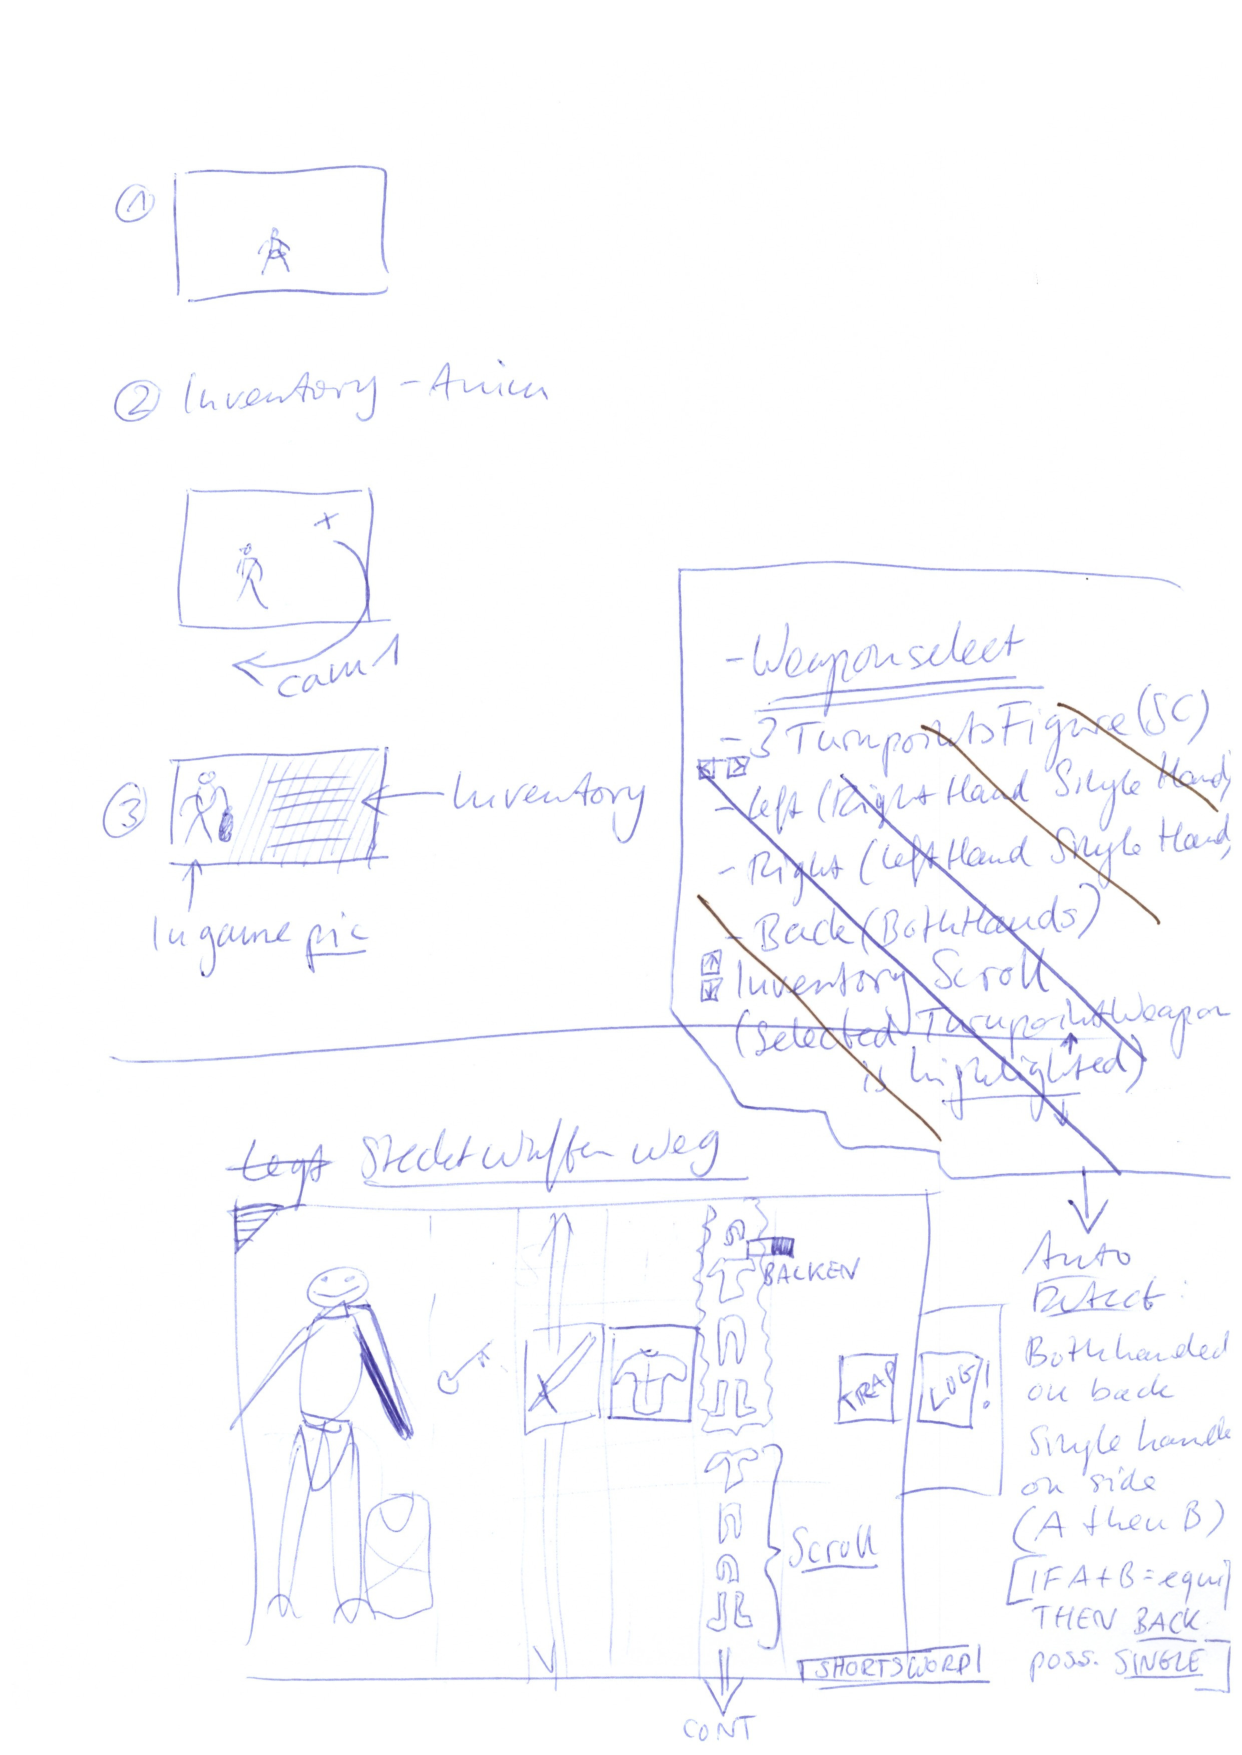
\includegraphics[scale=0.5]{orpheus_inventar.pdf}}
   \caption{Ausschnitt aus \enquote{\uline{\textsc{Orpheus} -- Interface}}}
   \label{fig:orpheus_inventar}
\end{figure}


%%%%%%%%%%%%%%%%%%%%%%%%%%%%%%%%%%%%%%%%%
% ORPHEUS – SPIELMECHANIK UND STEUERUNG %
%%%%%%%%%%%%%%%%%%%%%%%%%%%%%%%%%%%%%%%%%
\section{Spielmechanik und Steuerung}\label{sec:orpheus_mechanik}
Einige der oben genannten Dokumente befassen sich im weitesten Sinne mit spielmechanischen und steuerungsbezogenen Fragen, nämlich \enquote{Orpheus -- Interface} sowie die Notizen zur Kampfsteuerung.
Auch in dem Konvolut \enquote{Orpheus. B -- Scribbles} finden wir ein paar relevante Stichpunkte.
Wir werfen zuerst einen Blick auf einige generelle Überlegungen dazu, was es im Spiel geben sollte, wobei wir feststellen werden, dass natürlich nicht alle den Entwicklungsprozess überdauert haben.
Anschließend werden wir uns der Steuerung widmen, bevor wir...

Bei \enquote{\uline{\textsc{Orpheus} -- Interface}} handelt es sich um sieben mit (blauem) Kugelschreiber und (ursprünglich wahrscheinlich schwarzem, mittlerweile eher ins Braune tendierendem) Fineliner handbeschriebene Seiten,\footnote{Hinter dieser Überschrift ist mit rotem Fineliner -- wahrscheinlich von späterer Hand -- der Hinweis \enquote{V1} ergänzt worden. Anders als bei \enquote{\textsc{Orpheus} -- Spielwelt/Gildensystem} ist hier aber keine zweite Version erhalten.} auf denen einige grundlegende Designentscheidungen festgehalten sind.
An oberster Stelle auf der ersten Seite begegnen uns drei nummerierte Stichpunkte:
\enquote{\uline{Outside View Only}}, \enquote{\uline{Tastatur Only} (evtl Maus Inventory \& \enquote{\uline{Fernklick}} Unterstützung)} sowie \enquote{Items = VOBs},\autocite[S.~1]{orpheus_interface} wobei \enquote{VOB} hier für \enquote{Virtuelles Objekt} steht.\footnote{Zur Rolle von VOBs bei Gothic vgl. \autocite{wiki_vob}.}
Alle drei Punkte haben sich als für die Entwicklung von Gothic maßgeblich herausgestellt:
Den Namenlosen Helden sehen wir immer aus der Third-Person-Perspektive, die Steuerung unterstützt zwar Mauseingabe, bleibt in der Hauptsache aber auf die Tastatur fokussiert, und alle Gegenstände, die wir in der Spielwelt finden können, sind in der Engine als virtuelle Objekte angelegt.

Unter diesen drei wegweisenden Stichpunkten folgt eine von (a) bis (p) reichende Liste mit Dingen, die es im Spiel geben sollte:
\enquote{div[erse] Schläge}, \enquote{Zielen \& Schießen}, \enquote{Spell Selection}, \enquote{klettern}, \enquote{Springen}, \enquote{Türen öffnen/Truhe öffnen}, \enquote{Schloß knacken}, \enquote{ansehen}, \enquote{VOB verschieben}, \enquote{in VOB verstecken}, \enquote{Party NSC lenken}, \enquote{Battle Mode}, \enquote{reden}, \enquote{aufheben}, \enquote{Inventory} und \enquote{weglegen}.\autocite[S.~1]{orpheus_interface}
Das meiste davon ist am Ende auch umgesetzt worden; nur bei vier Punkten -- \enquote{VOB verschieben}, \enquote{in VOB verstecken}, \enquote{Party NSC lenken} und \enquote{Battle Mode} -- gibt es nennenswerte Abweichungen.

Nachdem Mike Hoge sich zu dieser Zeit noch die Frage \enquote{sollen \uline{alle} mögl. \uline{verschiebbar} sein?}\autocite[S.~3]{orpheus_interface} notiert hatte, ist \enquote{VOB verschieben} im fertigen Spiel -- wenn überhaupt -- nur noch als einzelnes, für Spieler*innen irrelevantes Artefakt vorhanden:
In der Klosterruine gibt es eine freistehende Säule, die sich zwar nicht wirklich verschieben, aber zumindest umwerfen lässt -- wobei sie dann auch noch in die falsche Richtung fällt.
Es scheint offensichtlich, das sie als improvisierte Brücke zur Überwindung eines Abgrunds dienen sollte.
Statt über den Abgrund fällt sie aber, wenn man sie umstößt, vom Abgrund fort.
Ob das schon als \enquote{verschieben} zählen darf, ist freilich diskutabel.
An die Idee, zum Beispiel einen \enquote{Schrank [$\ldots$] verschieben}\autocite[S.~3]{orpheus_interface} zu können, reicht es jedenfalls nicht mehr heran.

Ähnlich sieht es für den Stichpunkt \enquote{in VOB verstecken} aus:
Vereinzelt finden wir in der Spielwelt noch Fässer\footnote{Ein Objekt, das uns an verschiedenen Stellen in den Notizen begegnet, vgl. \autocite[S.~19]{orpheus_b_scribbles}, \autocite[S.~6]{orpheus_interface}.} -- eines im Alten Lager und zwei in der Alten Miene --, in denen sich unser Namenloser Held verstecken kann.
Eine spielmechanische Funktion erfüllen sie aber nicht.

Bei Gothic steht außerdem nur eine Spielfigur im Fokus und damit keine klassische Party, die sich aus verschiedenen Charakteren zusammensetzt.
Zwar gibt es vereinzelt Begleiter, mit denen man kurzfristig gemeinsam durch die Spielwelt streifen kann, steuern lassen sich diese allerdings -- wenn man von dem Zauber »Kontrolle« einmal absieht -- nicht. % Memo: Prüfen, ob das geht. %
\enquote{Party NSC lenken} ist im Laufe der Entwicklung also auch unter den Tisch gefallen.
Darauf, dass die Möglichkeit einer Party aber ernsthaft in Erwägung gezogen wurde, deuten einige weitere Notizen in \enquote{Orpheus -- Interface} hin.
\enquote{Bis zu 4 Party NSCs}\footnote{\autocite[S.~5]{orpheus_interface}. An anderer Stelle ist von \enquote{2 Slots (1 + 1)} die Rede (\autocite[S.~7]{orpheus_b_scribbles}).} sollte es geben.
Diese \enquote{Kontrollierte[n] NSCs [sollten] \uline{farblich} gekennzeichnet}\autocite[S.~5]{orpheus_interface} sein und sich über eine Reihe an Befehlen steuern lassen.
In einer kleinen Skizze sind dafür vier nebeneinanderliegende Tasten eines \enquote{Pop Up Menu[s]} mit \enquote{follow}, \enquote{wait}, \enquote{action} und \enquote{attack} beschriftet.\autocite[S.~3]{orpheus_interface}
An anderer Stelle finden wir eine abweichende Variante mit vier verschiedenen Knöpfen:
Über den \enquote{\uline{1. Button}} sollte ein kontrollierter Charakter dazu aufgefordert werden können, zu \enquote{Warte[n]} oder zu \enquote{Folge[n]}.
Eine dritte Option, nämlich ihn \enquote{\sout{Fliehe}[n]} zu lassen, ist hier durchgestrichen.
Über einen \enquote{\uline{2. Button}} sollte er dazu aufgefordert werden können, eine \enquote{Aktion} auszuführen, beispielsweise -- bezogen auf eine Tür -- \enquote{Lockpick} oder \enquote{Einrennen}.
Über einen \enquote{\uline{3. Button}} hätte man über \enquote{Kampf/Sparflamme} entscheiden können sollen, also wahrscheinlich darüber, ob der kontrollierte Charakter mit gezogener Waffe kampfbereit sein soll oder nicht.
Die Partymitglieder \enquote{kämpfen bis 15\%} ihrer Lebensenergie, hätten aber \enquote{\uline{Keine} selbstständige Aggression gegen andere NSCs}.
Über einen \enquote{General Button} schließlich hätte sich ein \enquote{Kriegsrat} der Party einberufen lassen sollen.
Diese Befehle hätten sich wahrscheinlich jeweils auf ein einziges Mitglied der Gruppe beziehen sollen.
Darauf könnte zum einen hindeuten, dass die Notiz so aussieht, als sollten die drei Buttons unter dem Balken für Lebensenergie erscheinen, der überlicherweise erscheint, wenn man sich einem NSC (oder einem Monster) zuwendet.
Außerdem sind zwei weitere -- danach wieder durchgestrichene -- Ideen für einen \enquote{\sout{General Button 2}} sowie einen \enquote{\sout{General Button 3}} notiert.
Mit ersterem hätte man zwischen \enquote{\sout{Alle Warten/Alle Folgen/Alle Kampf}} und mit zweiterem zwischen \enquote{\sout{Kampf/Alle Still}} umschalten können sollen;\autocite[S.~5]{orpheus_interface} \enquote{General} scheint sich also immer auf die ganze Gruppe zu beziehen.

Eine solche Party bringt andere spielmechanische Herausforderungen mit sich als ein einzelner Charakter:
Wenn unser Namenloser Held in Gothic stirbt, ist das Spiel zu Ende und wir müssen neu laden.
Aber wie geht man damit um, wenn nur ein Mitglied der Party stirbt?
\enquote{\textsc{Wie Wiederbelebung?}} fragt Mike Hoge an einer Stelle und notiert daneben, dass das über einen \enquote{\uline{Schrein}} geregelt werden könnte, der dem \enquote{Mafiabos} gehört.\autocite[S.~7]{orpheus_b_scribbles}
Die auf einer anderen Seite befindliche Notiz \enquote{\uline{1} XP Pool}\autocite[S.~8]{orpheus_b_scribbles} könnte sich wiederum darauf beziehen, dass Erfahrungspunkte nicht für jedes Partymitglied einzeln, sondern für die Gruppe als ganzes gezählt werden sollen.
Ein ähnliches Problem gibt es für die Objekte, die sich in der Spielwelt sammeln lassen:
\enquote{Individuell \textsc{oder} Gruppe} schreibt Mike Hoge unter der Überschrift \enquote{\uline{Besitzflag}}.
Es lässt sich vermuten, dass jedes Objekt entweder als Besitz eines Charakters oder als das der Party ausgewiesen werden sollte, wobei gilt:
\enquote{08/15 Items haben Gruppenflag.}\autocite[S.~9]{orpheus_b_scribbles}
Außerdem stellt sich -- darauf deutet der Stichpunkt \enquote{Partymitglied\_Bewegungs\_Spielraum}\autocite[S.~8]{orpheus_b_scribbles} hin -- die Frage, wie mit räumlicher Entfernung zwischen den einzelnen Partymitgliedern umgegangen werden soll.
Es gibt beispielsweise Überlegungen, dass die oben erwähnte Aufforderung \enquote{Folge} nicht funktionieren sollte, wenn sich ein Gruppenmitglied \enquote{außer Hörreichweite} befindet.
Weil das unter Umständen aber zu unpraktisch sein könnte, ist dazu in Klammern eine Alternative notiert:
\enquote{evtl Telepath. Kommunikation}.\autocite[S.~5]{orpheus_interface}
Und was macht man, wenn sich ein Gruppenmitglied -- aber nicht der Spieler selbst -- an einem Ort aufhält, an dem etwas Wichtiges ausgelöst werden soll?
Der etwas kryptische Vermerk \enquote{Kritische Dialoge \textsc{nicht} Triggern wenn \uline{Party} $-$ NSC $=$ \uline{Mensch}!}\autocite[S.~9]{orpheus_b_scribbles} könnte unter Umständen so gelesen werden, dass ein wichtiger Dialog nicht ausgelöst werden soll, wenn Teile der Gruppe zwar am entsprechenden Ort sind, der menschliche Spieler (\enquote{NSC = Mensch}) aber fehlt (\enquote{$-$}); wobei man freilich darüber hinwegsehen müsste, dass \enquote{NSC} eigentlich einen Charakter beschreibt, der nicht der Spieler ist.

Neben \enquote{VOB verschieben}, \enquote{in VOB verstecken} und \enquote{Party NSC lenken} bleibt dann noch der \enquote{Battle Mode}, wobei nicht unmittelbar klar ist, was sich die Entwickler zu diesem Zeitpunkt darunter vorgestellt haben.
Bei der Erwähnung eines solchen Kampfmodus mag einem zum Beispiel der unter anderem in JPRGs bis heute tradierte Kampfbildschirm in den Sinn kommen, in dem das (in der Regel rundenbasierte) Geschehen oft abstrahiert aus einem Blick von der Seite dargestellt wird, wobei sich die Kontrahenten beispielsweise am linken und rechten Rand des Bildschirms oder diagonal gegenüberstehen.\footnote{Ein frühes -- vielleicht sogar das erste -- Beispiel für eine Kampfansicht, in der sich die Parteien links und rechts gegenüberstehen, stellt das 1987 in Japan und 1990 in den Vereinigten Staaten erschienene \textit{Final Fantasy} dar. Eine diagonale Gegenüberstellung findet sich etwa in dem 1993 erschienenen \textit{Ogre Battle -- The March of the Black Queen}. Daneben gibt es noch die frontale Darstellung der Gegner, entweder aus der Egoperspektive des Spielers, wie etwa im 1986 veröffentlichten \textit{Dragon Quest}, oder über die Schulter der Spielfiguren, wie beispielsweise im 1993 erschienenen \textit{Lufia \& the Fortress of Doom}. Diese Formen eines separaten Kampfbildschirms haben sich bis heute erhalten, etwa im 2016 erschienenen \textit{Persona 5} oder im 2018 erschienenen \textit{Octopath Traveler}.}
Und tatsächlich sehen wir in einer frühen Entwicklungsversion von Gothic, dass sich die Kamera im Falle eines Kampfes zur Seite bewegt und das Geschehen aus einer statischeren Perspektive zeigt, die nicht mehr strikt dem Charakter folgt, sondern sich nur verschiebt, wenn dieser sich hinreichend weit von seiner ursprünglichen Position entfernt.\footnote{Das ist der Fall in Version 0.56c; vgl. bspw. \autocite[Min.~5:11]{alpha_features}.}
Generell haben die frühen Überlegungen zum Kampf einen etwas taktisch anmutenden Charakter.
In \enquote{Orpheus -- Interface} ist die Idee festgehalten, dass man nach dem \enquote{Ausholen} (über \enquote{Fire}) mit \enquote{$\leftarrow$} und \enquote{$\rightarrow$} ein Ziel auswählen (\enquote{Select Target}), sich diesem dann mit \enquote{$\uparrow$} und \enquote{$\downarrow$} \enquote{nähern/entfernen} und schließlich über eine Auswahl zwischen \enquote{1} und \enquote{9} auf dem Ziffernblock eine Angriffsform auswählen kann (\enquote{Select Blow}).\autocite[S.~2]{orpheus_interface}
Die Notizen zur Kampfsteuerung lesen sich ähnlich taktisch.
Zentral ist bei den dort festgehaltenen Überlegungen die Distanz zum Gegner und wie sich diese durch die eigene Bewegung (etwa durch einen Angriff mit Ausfallschritt nach vorne oder durch eine Parade mit Schritt nach hinten) und die Bewegung des Gegners (etwa durch ein Zurückweichen beim Getroffenwerden) verändert.\autocite[Vgl.][S.~1--3]{orpheus_kampfsteuerung}
In einer Tabelle ist minutiös festgehalten, welche Art von Angriff welche Auswirkungen auf einen Gegner in welcher Distanz haben soll.\footnote{Vgl. \autocite[S.~4--5]{orpheus_kampfsteuerung}.}
Dabei wird unterschieden zwischen vier für den Nahkampf relevanten Distanzen, vier möglichen Tastatureingaben (\enquote{\textsc{Ctrl}} in Kombination mit \enquote{$\uparrow$}, \enquote{$\rightarrow$}, \enquote{$\leftarrow$} oder \enquote{$\downarrow$}) sowie einem Angriff mit der \enquote{Faust} oder mit einer von drei Waffen (\enquote{Dolch}, \enquote{Schwert} und \enquote{Zweihänder}), mit denen man entweder geübt oder ungeübt sein kann, was in einer Tabelle mit immerhin 112 Zellen resultiert.\autocite[S.~4]{orpheus_kampfsteuerung}

Im fertigen Spiel machen wir uns durch Drücken der Leertaste Kampfbereit.
Diese Idee ist schon in \enquote{Orpheus -- Interface} angelegt, wo notiert ist, dass durch einmaliges Drücken das Schwert gezogen und durch zweimaliges Drücken der Bogen bereit gemacht werden sollte.\autocite[S.~2]{orpheus_interface}
Mit gezogener Waffe (oder gehobenen Fäusten, wenn wir keine Waffe ausgerüstet haben) können wir dann durch die Steuerungstaste (kurz Strg) im Kombination mit W, A oder D angreifen, während uns Strg und S blocken lässt.
Diese Kombination von Steuerungs- und Richtungstasten geht -- wie wir oben im Zusammenhang mit der Tabelle gesehen haben -- ebenso auf diese frühe Phase zurück.
Den Notizen zur Kampfsteuerung zufolge sollte durch die Kombination von Strg und Pfeiltasten entweder unterschiedliche Gegner angegriffen oder verschieden Schwertstreiche auf den gleichen Gegner ausgeführt werden können.\footnote{Vgl. \autocite[S.~1--3]{orpheus_kampfsteuerung}; siehe auch \autocite[S.~4]{orpheus_interface}, wo wir ein Raster aus 3 × 3 Tasten finden, die in Kombination mit \enquote{Fire} jeweils unterschiedliche Aktionen im Kampf bewirken sollten. Von link nach Rechts sind das in der obersten Reihe \enquote{Tritt}, \enquote{Stechen} und Schlag von \enquote{Oben}, in der mittleren Reihe \enquote{L[inks] Seitlich [schlagen]}, \enquote{Barbarenschlag} und \enquote{R[echts] Seitlich [schlagen]} sowie in der unteren Reihe \enquote{L[inks] Rumgehen}, \enquote{Hinter Schlag} und \enquote{R[echts] Rumgehen}. Dieses Raster ist schon auf S.~1 hinter Punkt (a) \enquote{div[erse] Schläge} angedeutet.}

Auch abseits des Kampfes war Gothic schon immer für seine etwas eigenwillige Steuerung bekannt.
Petra Schmitz, die das Spiel vor seiner Veröffentlichung für die \textit{GameStar} bei einem Preview-Termin anspielen konnte, erinnert sich daran, wie schockiert sie davon war, dass das Spiel zu diesem Zeitpunkt keine Maussteuerung unterstütze.\autocite{schmitz_maussteuerung}
Die oben erwähnte Notiz \enquote{\uline{Tastatur Only}}\autocite[S.~1]{orpheus_interface} sollte bis zum Schluss richtungsweisend bleiben.
Ein zentrales Element der Steuerung im finalen Gothic ist auch außerhalb des Kampfes die Steuerungstaste.
Während die Bewegung klassisch über die Tasten W, A, S und D funktioniert, gesellt sich Strg hinzu, wenn wir mit Elementen in der Spielwelt interagieren wollen.
Drücken wir beispielsweise Strg und W, können wir unter anderem ein Objekt benutzen, einen Gegenstand aufsammeln, eine Truhe öffnen oder eine Person ansprechen.
In der Zeit von Orpheus sind solche Dinge noch auf verschiedene Tastenkombinationen verteilt.
\enquote{Fire + $\uparrow$} war für das \enquote{\uline{Manipulieren}} von Objekten in der Spielwelt (\enquote{Tür/Schrank/Truhe/Hebel/Knopf/Fackel}), \enquote{Fire + $\downarrow$} für das \enquote{\uline{Aufheben}} von Gegenständen (wobei man anschließend mit \enquote{up} oder \enquote{down} hätte entscheiden können sollen, ob man den Gegenstand ins Inventar aufnehmen oder \enquote{wieder weglegen} möchte), \enquote{Fire + $\leftarrow$} für das \enquote{\uline{Betrachten}} und \enquote{Fire + $\rightarrow$} für das \enquote{\uline{Reden}} gedacht.\autocite[S.~2]{orpheus_interface}
Daneben war \enquote{Alt} für \enquote{Springen/Klettern/in VOB verstecken} vorgesehen.\autocite[S.~3]{orpheus_interface}

Die Notizen zur Auswahl von Zaubern wiederum sind etwas kryptisch.
Es scheint, als sei die erste Idee gewesen, dass man über eine Funktion zum Schnellzugriff mittels der Tabulatortaste auf verschiedene Gegenstände hätte zugreifen können sollen, wobei eines davon das Zauberbuch gewesen wäre (\enquote{QuickSlot2 $=$ SpellBook; $\rightleftarrows$<\textsc{tab}> $=$ Get\uline{QS2}items}).
Über \enquote{Fire} hätte sich dann ein Spruch aus dem Buch vorbereiten lassen sollen (\enquote{<Fire> $=$ \uline{Activate} [Bookmark] Spell}).
Darunter ist notiert, dass sich das Buch auch über die Eingabetaste hätte öffnen lassen (\enquote{<Return> $=$ Book $\Rightarrow$ Spell Select (Bookmark)}) und sich eine Auswahl an Zaubern unter Umständen auf den Nummernblock hätte legen lassen (\enquote{evtl. QuickChoiceSpells on Keypad 1--0}) sollen.
Es scheint damit so, dass man sich zuerst einen Zauber aus seinem Buch hätte zurechtlegen müssen, ehe man ihn dann -- in einem nächsten Schritt -- hätte wirken können.
Von späterer Hand sind allerdings zwei Notizen hinzugefügt worden, die darauf hinzudeuten scheinen, dass sich -- entweder auch oder stattdessen -- ohne den Umweg über das Zurechtlegen \enquote{\textsc{direkt aus} [dem] \textsc{Buch zaubern}} lassen sollte, indem man zunächst die Eingabetaste drückt, dann denn Zauber auswählt und ihn dann mit \enquote{Fire} wirkt (\enquote{<Return>$_{\downarrow}^{\uparrow}$<Fire>}).
Neben diesen Überlegungen zur Steuerung finden wir an dieser Stelle zwei generelle Gedanken zu Zaubern:
Sie sollten, erstens, einer \enquote{\textsc{\uline{logische}}[n] \textsc{\uline{Sortierung}}} folgen und, zweitens, sollte es \enquote{\textsc{wenig Sprüche auf einmal}} geben, die dafür aber über eine \enquote{\textsc{individuelle $[\dots]$ Steigerung}} verfügen sollten, indem man die entsprechende Taste länger gedrückt hält (darauf deuten die beiden Vermerke \enquote{long press mighty spell} und \enquote{<Fire\_pressed> $=$ Inc[line] Spell Strength} hin).\autocite[S.~3]{orpheus_interface}


%%%%%%%%%%%%%%%%%%%%%%%%
% ORPHEUS – GESCHICHTE %
%%%%%%%%%%%%%%%%%%%%%%%%
\section{Geschichte}\label{sec:orpheus_geschichte}


%%%%%%%%%%%%
% APPENDIX %
%%%%%%%%%%%%
\clearpage
\appendix


%%%%%%%%%%%%%%%%
% BIBLIOGRAFIE %
%%%%%%%%%%%%%%%%
\clearpage
\printbibliography

\end{document}
